\documentclass[final]{beamer}

\usepackage[size=custom, width=36, height=24, scale=0.36]{beamerposter}
\usetheme{gemini}
\usecolortheme{msu}
\usepackage[labelfont=bf]{caption}
\usepackage{picins}

\newlength{\sepwidth}
\newlength{\colwidth}
\setlength{\sepwidth}{0.025\paperwidth}
\setlength{\colwidth}{0.3\paperwidth}

\newcommand{\separatorcolumn}{\begin{column}{\sepwidth}\end{column}}

\title{High-Throughput Phenotyping using Computer Vision and Machine Learning}

\author{Vivaan Singhvi, Langalibalele Lunga, Pragya Nidhi, Chris Keum, Varrun Prakash}

\institute{Farragut High School}

\footercontent{
    \href{https://github.com/vivaansinghvi07/smoky-mountain-data-comp}{Github: vivaansinghvi07/smoky-mountain-data-comp} 
    \hfill
    Smoky Mountains Computational Sciences Data Challenge Conference 
    \hfill
    \href{mailto:singhvi.vivaan@gmail.com}{singhvi.vivaan@gmail.com}
}

\begin{document}

\begin{frame}[t]
\begin{columns}[t]
\separatorcolumn

\begin{column}{\colwidth}

\begin{block}{Introduction and Background Information}

% ---------------------------------------------------- % 

\textbf{High-throughput phenotyping} is a breakthrough technology used in plant biology and agriculture to examine a wide variety of plant features through \textbf{image analysis}. By coupling this technique with \textbf{machine learning}, scientists can handle plant datasets \textbf{thousands of times larger} in a \textbf{fraction of the time}.

% ---------------------------------------------------- % 

\end{block}

\begin{alertblock}{Research Objective}

% ---------------------------------------------------- % 

Using a dataset of \textbf{1672} images (with spanning \textbf{white labels}) of the plant \textbf{Populus Trichocarpa}, provided by Oak Ridge National Laboratory, we aim to address the following summarized challenge questions:

% ---------------------------------------------------- % 

\begin{enumerate}
    
    \item Is it possible to use \textbf{optical character recognition} to “read” each label and \textbf{generate a spreadsheet} of the features on the label?
    \item Can \textbf{machine learning} classify different \textbf{leaf morphologies} among plants, such as leaf shape or color?
    \item Can a \textbf{predictive model} be built \textbf{using leaf morphology classifications} that can indicate the \textbf{condition} in which a plant was raised?
    \item GPS and other camera information are encoded in \textbf{EXIF tags}. Can this data be used to determine characteristics such as leaf size? Can other data, such as soil maps, weather, etc. be used to find \textbf{correlations among phenotypes}?

\end{enumerate}

% ---------------------------------------------------- % 

\end{alertblock}

\begin{block}{Reading Labels with Optical Character Recognition}

% ---------------------------------------------------- % 

\begin{itemize}
    \item The prebuilt model \textbf{PaddleOCR} was chosen for label reading due to its \textbf{accuracy} and \textbf{efficiency}.
    \item However, minor \textbf{image augmentation} was needed to configure images, including \textbf{edge highlighting} and \textbf{rotating}.
\end{itemize}

% ---------------------------------------------------- % 


\begin{center}
    \includegraphics[width=0.87\colwidth]{images/step1_pipeline.png}
    \captionof{figure}{The image augmentation process for optical character recognition}
\end{center}

\vspace{-0.5\intextsep}

% ---------------------------------------------------- % 

\begin{itemize}
    \parpic(0px, 0px)(0px, 1.7cm)[r]{
        \resizebox{0.57\colwidth}{!}{
            \begin{minipage}{\colwidth}
                \captionsetup{font={Large}}
                \begin{tabular}{|c|c|c|c|c|c}
                     \hline
                     filename & treatment & block & row & position & genotype \\
                     \hline
                        ... & D & 1 & 8  & 32 & BESC-34 \\
                        ... & C & 1 & 10 & 12 & **BESC-417\_LM**,core \\
                        ... & C & 2 & 3  & 40 & BESC-468 \\
                        ... & C & 2 & 6  & 54 & BESC-28\_LM \\
                        ... & C & 1 & 24 & 22 & **LILD-26-5\_LM**,core \\
                        ... & 	& 	& 	 &	  & **HOMD-21-2\_LM**,core \\
                        ... & C	& 2	& 23 & 45 & BESC-361\_16\_11\_CB \\
            	      ... &   & 1 & 25 & 30	& **BESC-106\_LM**,core \\
                     \hline
                \end{tabular}
                \captionof{table}{Example spreadsheet data}
            \end{minipage}
        }
    }
    \item \textbf{Regular Expressions} extracted features from text.
    \item On 30 random images, the model had an accuracy of \textbf{77.33\%}, \textbf{94.31\%} with null values omitted.
\end{itemize}

% ---------------------------------------------------- % 


\end{block}

\end{column}

\separatorcolumn

\begin{column}{\colwidth}

\begin{block}{Classifying Leaf Morphologies with Image Segmentation}

% ---------------------------------------------------- % 

\begin{itemize}
    \item The \textbf{Segment Anything Model} (SAM) was chosen to segment leaves. The \texttt{SamPredictor} could generate an exact mask at a \textbf{given point}.
    \item To approximate these points, the below pipeline was used, using \textbf{HSV Filtering}, \textbf{Edge Detection}, and \textbf{Dilation} techniques.
\end{itemize}

% ---------------------------------------------------- % 

\vspace{-1em}

\begin{center}
    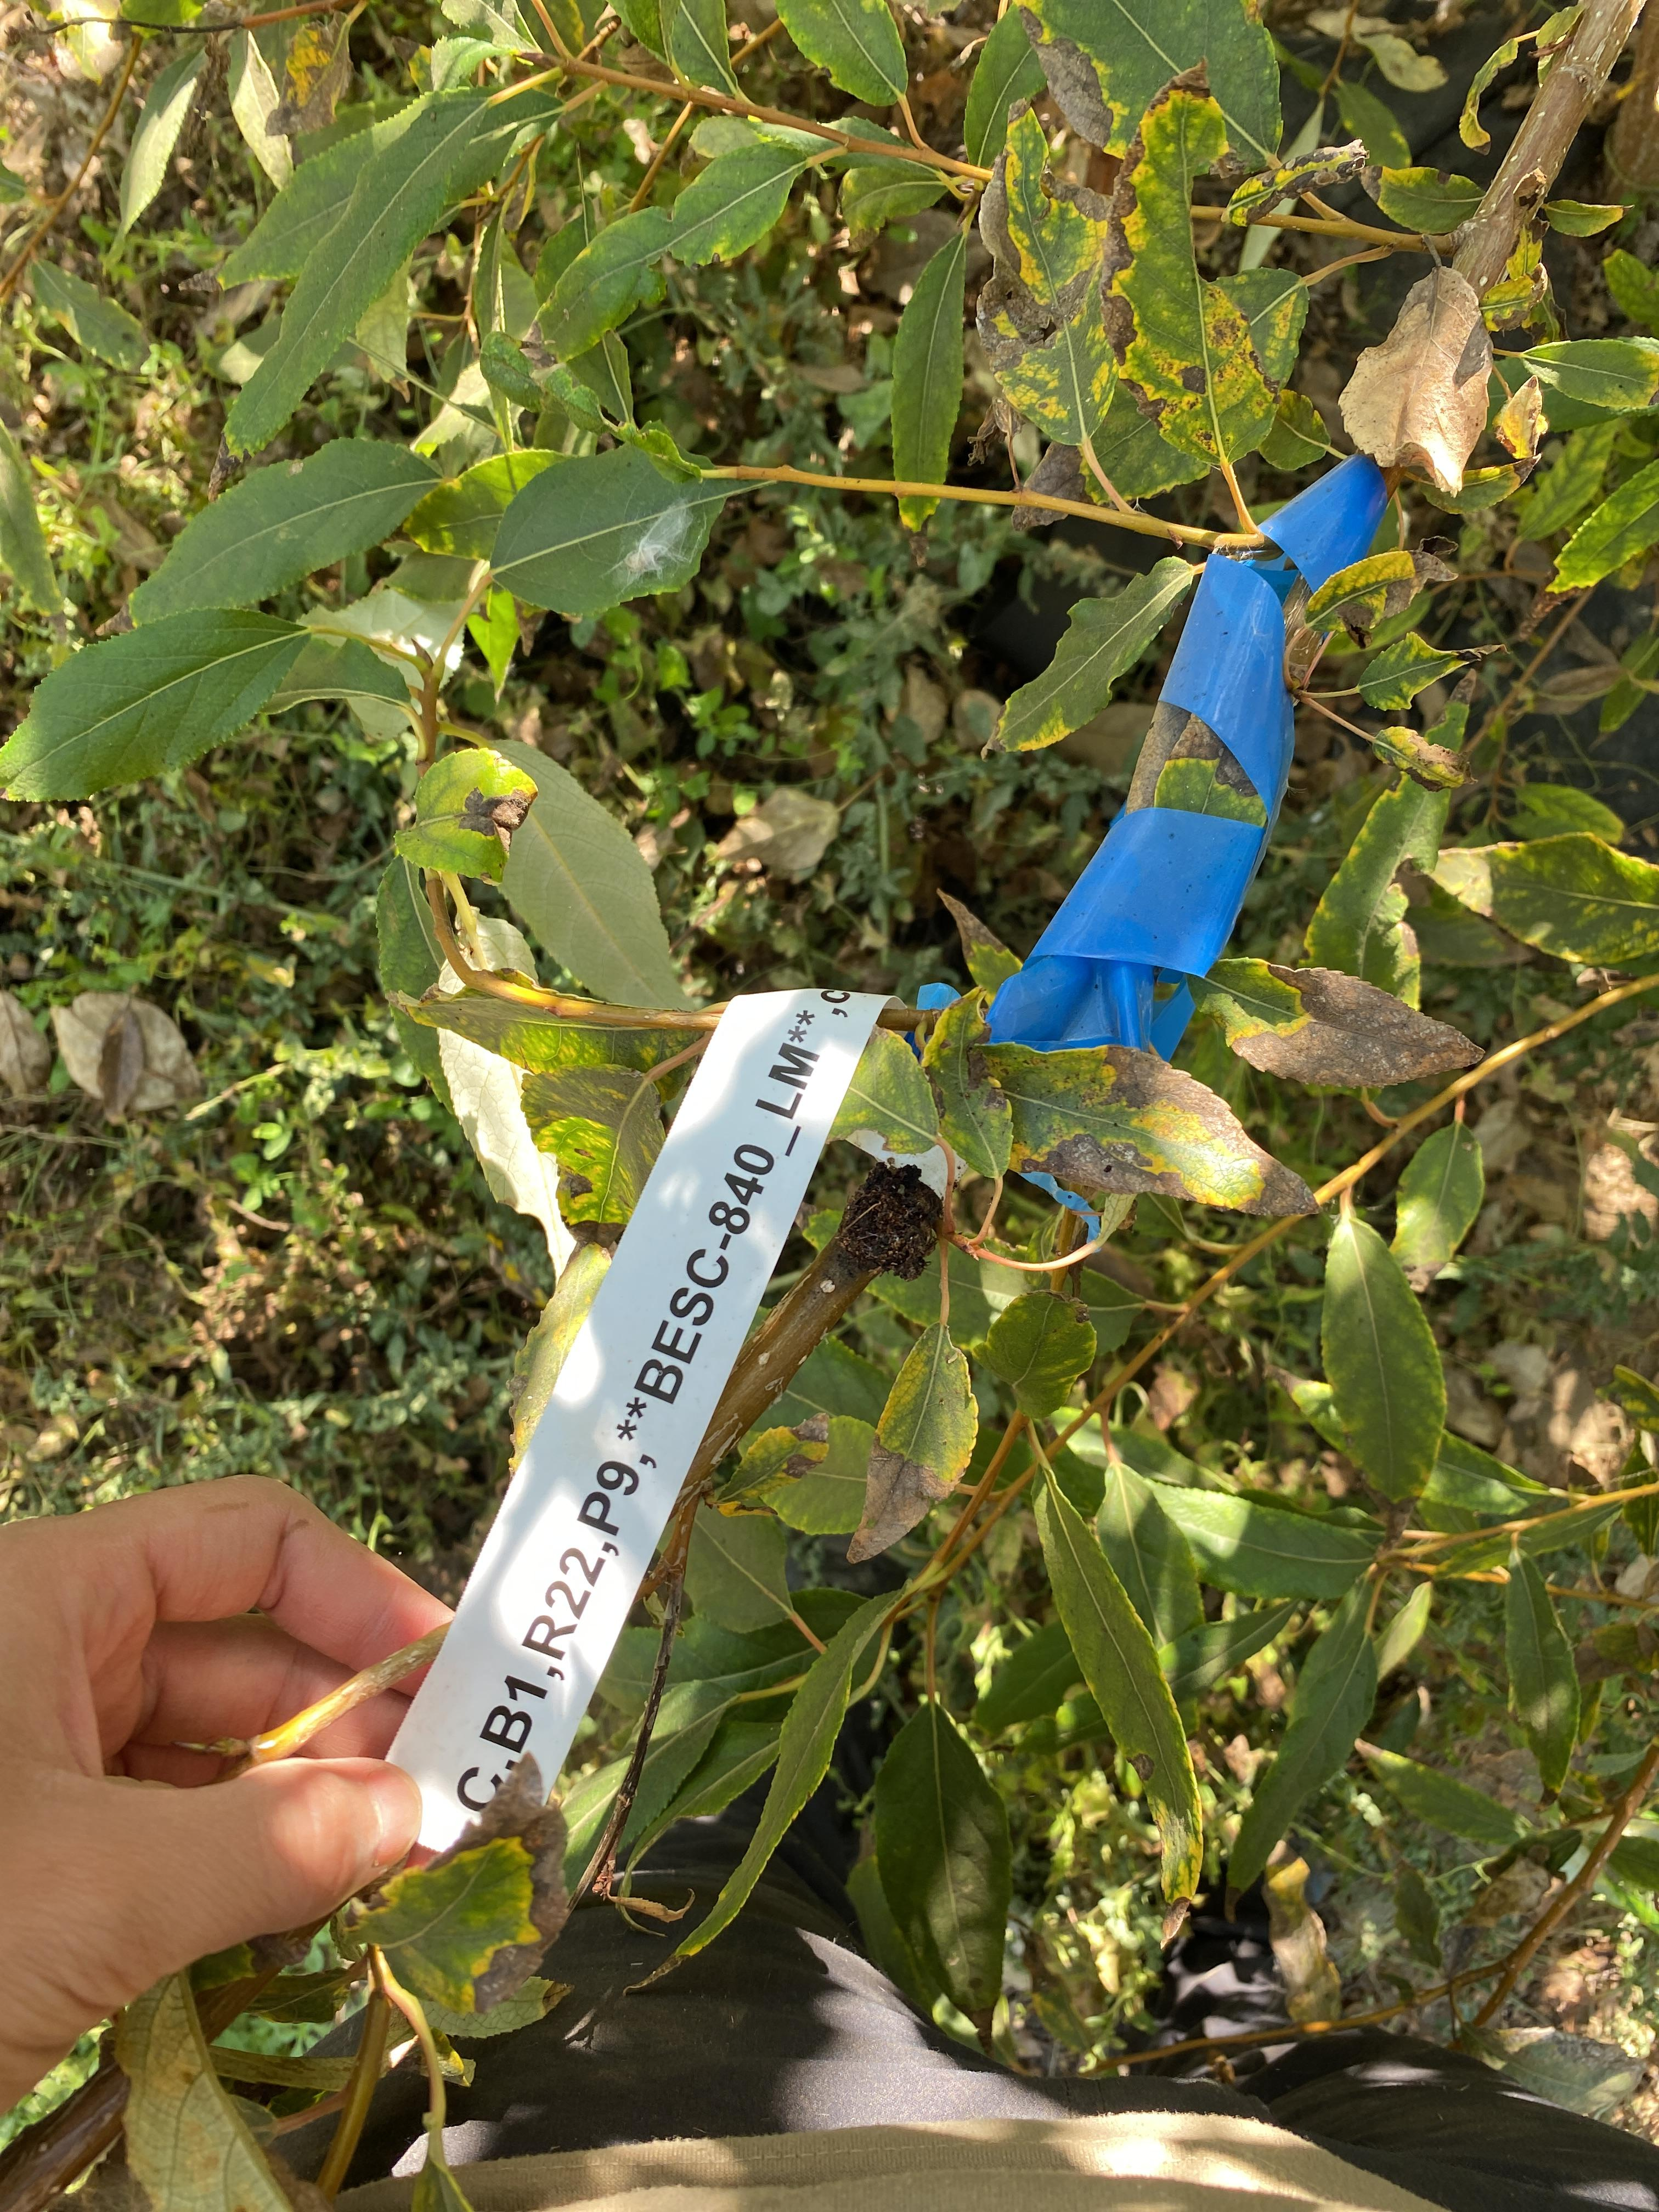
\includegraphics[width=0.22\colwidth]{1.png}
    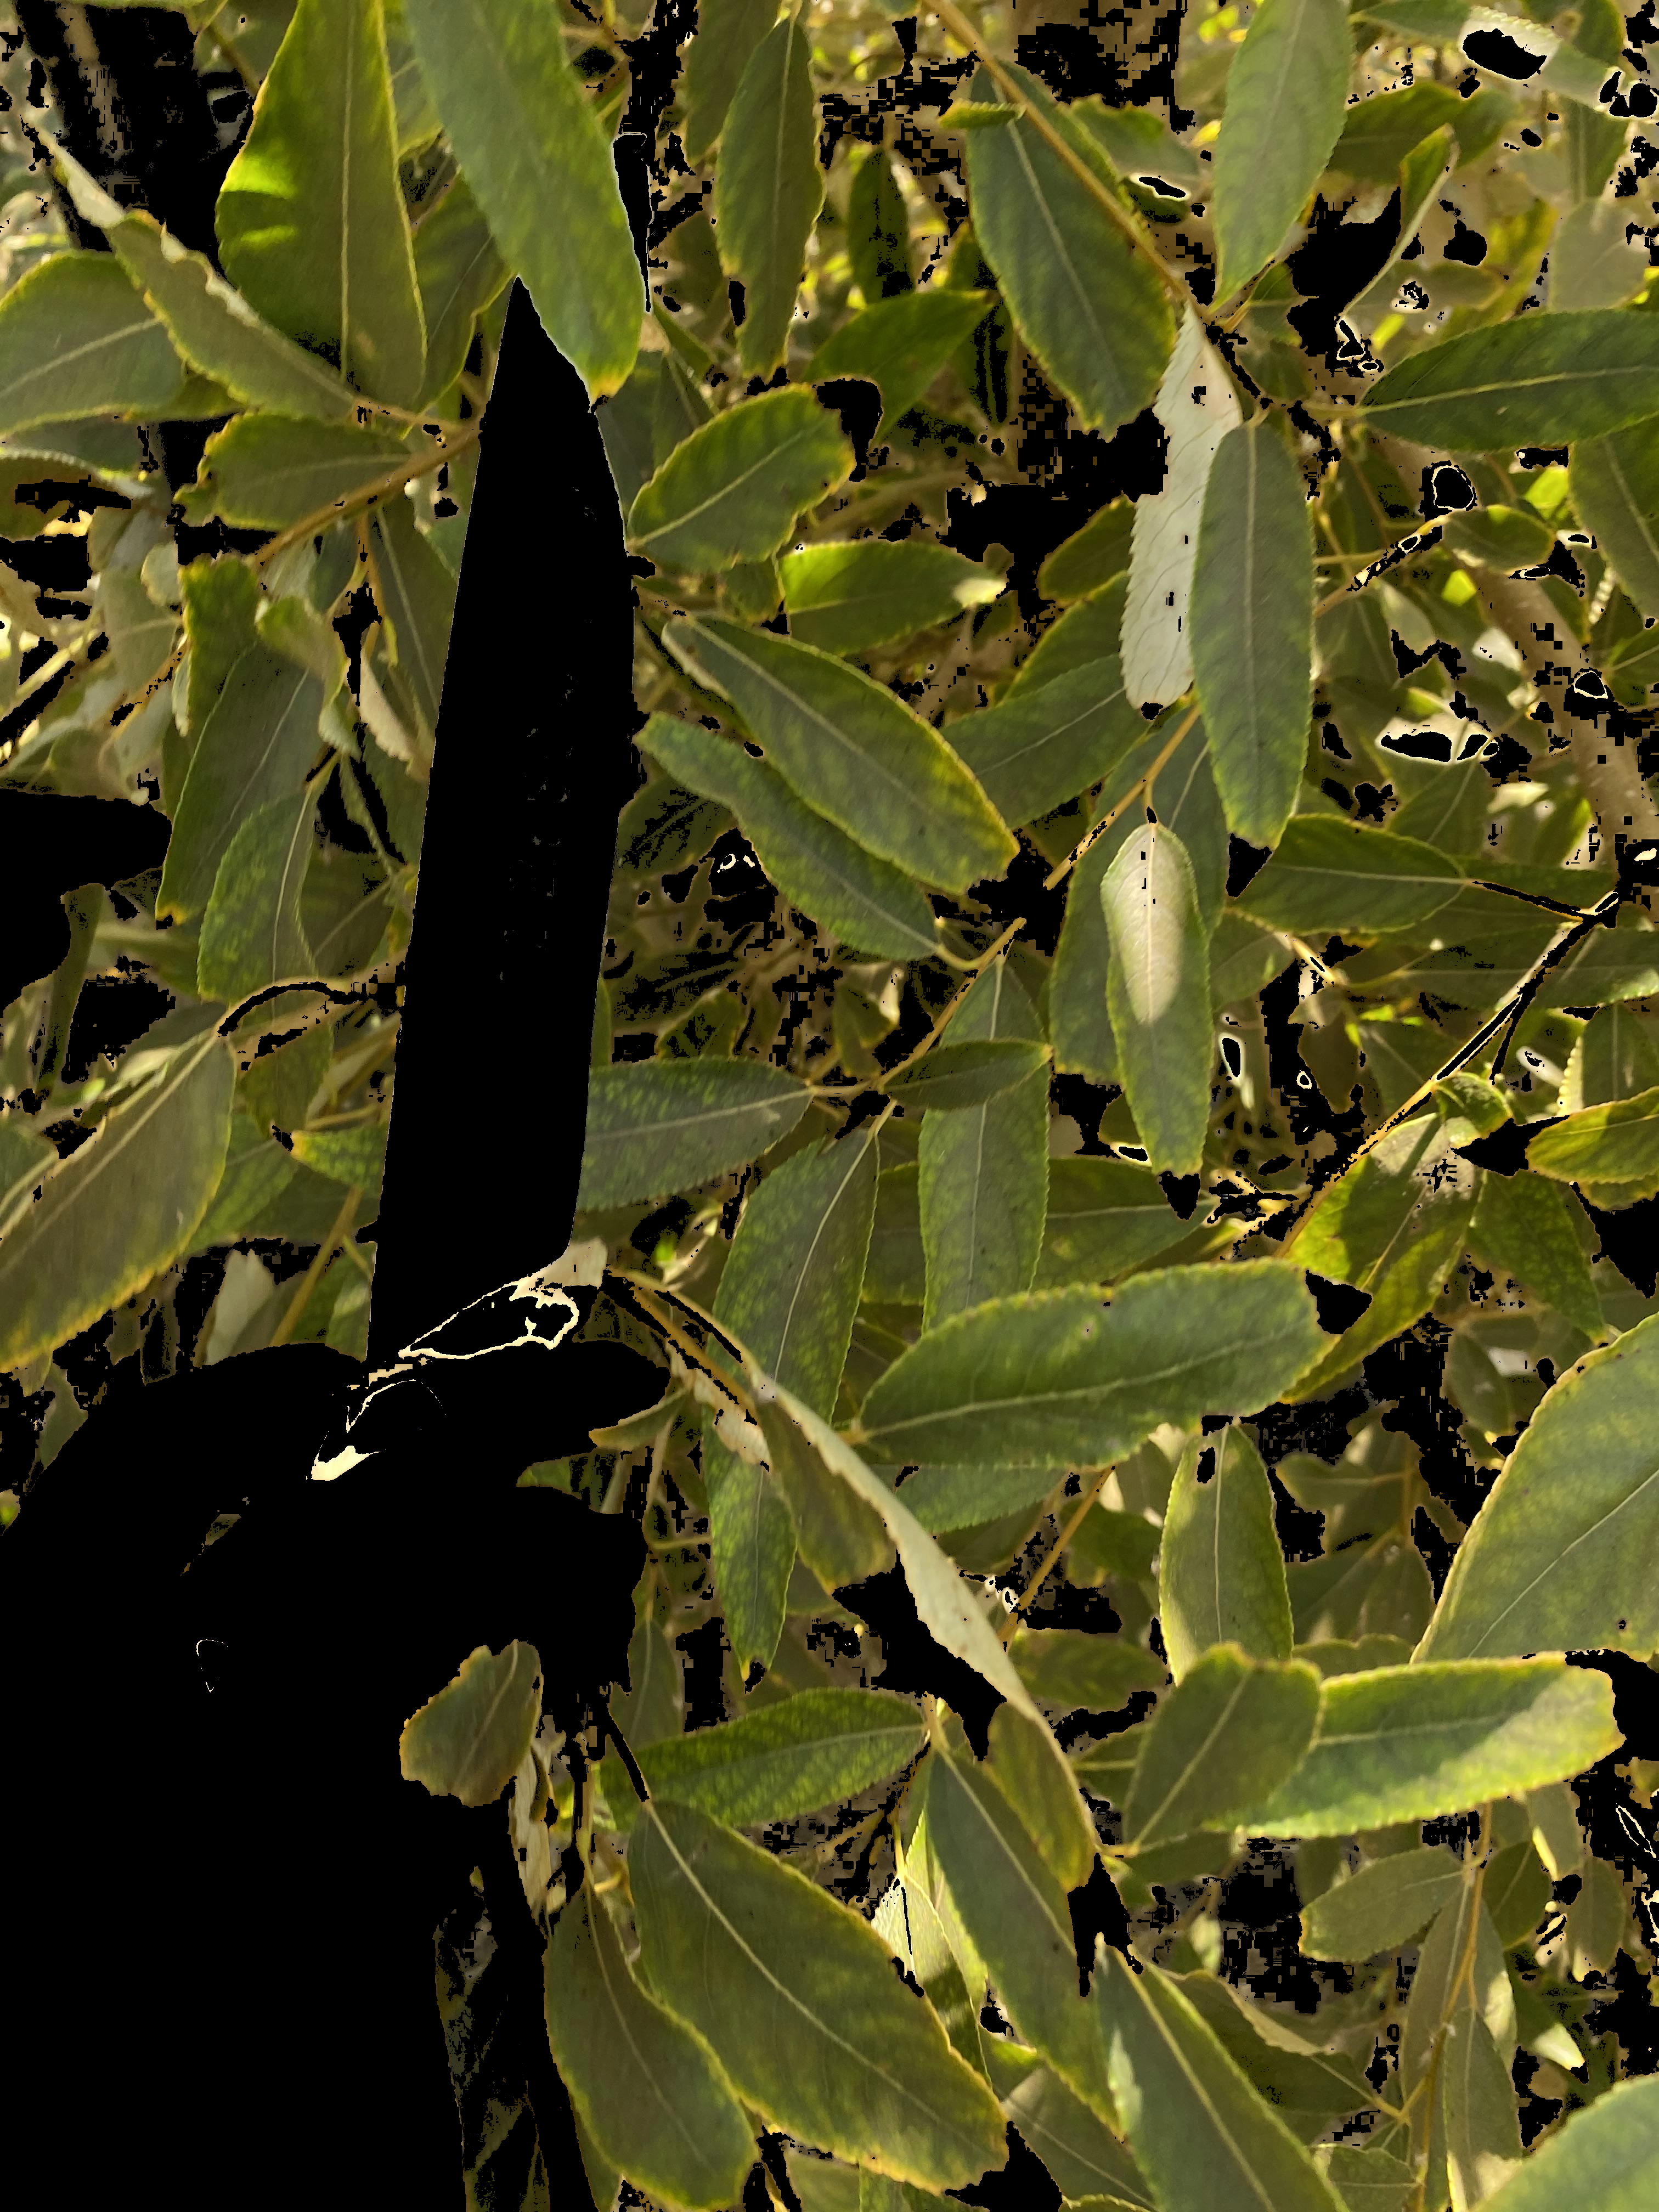
\includegraphics[width=0.22\colwidth]{2.png}
    \includegraphics[width=0.22\colwidth]{4.png}
    \includegraphics[width=0.22\colwidth]{6.png}
    \captionof{figure}{The image processing pipeline utilized to generate leaf approximations}
\end{center}

\vspace{-0.5\intextsep}

% ---------------------------------------------------- % 

\vspace{-0.7em}

\begin{itemize}
    \parpic(0px, 0px)(0px, 2.75cm)[l]{
        \begin{minipage}{0.28\colwidth}
            \includegraphics[width=0.28\colwidth]{images/2_better.png}
            \captionof{figure}{Segmentation masks after filtering}
        \end{minipage}
    }
    \item The \textbf{centers} of these approximations were used as the \textbf{generation point}.
    \item Then, using a \textbf{machine learning classifier}, we \textbf{filtered bad segmentations} (shown in red to the left) with an accuracy of \textbf{90.91\%}.
    \item The masks are then used to \textbf{classify morphologies}.
    \item The chosen features were \textbf{color}, \textbf{shape}, and \textbf{level of brown splotch} (indicating withering leaves).
    \item The \texttt{XGBoost} model classified the features, and \texttt{scikit-learn}'s \texttt{MultiOutputClassifier} was implemented to manage all three at once.
\end{itemize}

% ---------------------------------------------------- % 

\vspace{-0.5em}

\begin{center}
    \includegraphics[width=0.32\colwidth]{images/color.png}
    \includegraphics[width=0.32\colwidth]{images/shape.png}
    \includegraphics[width=0.32\colwidth]{images/splotch.png}
    \captionof{figure}{Confusion matrices for color, shape, and splotch respectively}
\end{center}

% ---------------------------------------------------- % 

\vspace{-1em}

\begin{itemize}
    \item The \textbf{color} classifier had an accuracy of \textbf{69.23\%}, and seemed to be confused around \textbf{true yellow-green} leaves.
    \item The \textbf{shape} classifier was more sporadic with an accuracy of \textbf{50.00\%}, \textbf{mispredicting} \textbf{oblong} and \textbf{ovate} leaves the most.
    \item The \textbf{splotch} classifier had an accuracy of \textbf{69.23\%}, without significant errors.
    \item The model was used on \textbf{every image} by finding the \textbf{mode prediction} for each feature. Then, this data was \textbf{inserted into the spreadsheet}. 
\end{itemize}

% ---------------------------------------------------- % 

\end{block}

\end{column}

\separatorcolumn

\begin{column}{\colwidth}

\begin{block}{Predicting Treatment from Morphological Classifications}

% ---------------------------------------------------- % 

\begin{itemize}
    \item By using \textbf{read treatments} from step 1 in conjunction with \textbf{morphological classifications} from step 2, we could build a simple predictor to determine if a plant was raised in \textbf{drought} or \textbf{control}.
\end{itemize}

\vspace{-1em}

% ---------------------------------------------------- % 

\begin{itemize}
    \parpic(0px, 0px)(0px, 1.3cm)[r]{
        \resizebox{0.57\colwidth}{!}{
            \begin{minipage}{\colwidth}
                \begin{tabular}{|c||c c c c|} 
                     \hline
                     leaf\_color & light\_green & dark\_green & yellow\_green & yellow  \\
                     \hline
                     light\_green & 1 & 0 & 0 & 0 \\
                     yellow\_green & 0 & 0 & 1 & 0 \\
                     dark\_green & 0 & 1 & 0 & 0 \\ 
                     light\_green & 1 & 0 & 0 & 0 \\
                     yellow & 0 & 0 & 0 & 1 \\
                     \hline
                \end{tabular}
                \captionsetup{font={Large}}
                \captionof{table}{Example of one-hot encoding}
            \end{minipage}
        }
    }
    \item \textbf{One-hot encoding}, as seen to the right, was used to convert our \textbf{qualitative} data to \textbf{quantitative} data.
\end{itemize}

% ---------------------------------------------------- % 

\begin{itemize}
    \parpic(0px, 0px)(-0.2cm, 2.6cm)[l]{
        \begin{minipage}{0.35\colwidth}
            \includegraphics[width=0.35\colwidth]{images/treat_conf_matrix.png}
            \captionof{figure}{Confusion matrix for treatment classifier}
        \end{minipage}
    }
    \item Some data had to be \textbf{pruned} as to avoid \textbf{class imbalance}.
    \item Our model, a \texttt{RandomForestClassifier}, had an accuracy of \textbf{60.08\%} and a confusion matrix shown on the left.
    \item The low accuracy is likely due to our limitation of \textbf{only using classification data} from the previous step. Along with the fact that they \textbf{may be inaccurate}, only three features are \textbf{likely not enough} to make good predictions.
\end{itemize}

% ---------------------------------------------------- % 

\end{block}

\vspace{1em}

\begin{block}{Finding Correlations and Characteristics from EXIF Tags}

% ---------------------------------------------------- % 

\begin{itemize}
    \item The EXIF tags were \textbf{not useable} for predicting leaf size, or other traits. 
    \item A vital tag, the \texttt{FocalPlaneResolution}, was \textbf{missing} from the images.
    \item Additionally, since all leaves were close together, \textbf{no weather or soil map API} would provide geolocational data \textbf{specific enough} for us.
    \item If this information were \textbf{present in a given file}, we could make conclusions.
\end{itemize}

% ---------------------------------------------------- % 

\end{block}

\begin{exampleblock}{Conclusion and Significance}

% ---------------------------------------------------- % 

\begin{itemize}
    \item We were \textbf{successfully} able to read plant labels with \textbf{optical character recognition} and store the data in our spreadsheet. 
    \item We were \textbf{successfully} able to extract leaves from the images and \textbf{somewhat successfully} able to classify their \textbf{morphologies}.
    \item We were \textbf{slightly successfully} able to determine \textbf{treatment} from morphology classifications and \textbf{not successful} in making conclusions from \textbf{EXIF tags}.
    \item Regarding \textbf{originality}, this study is \textbf{one of the first} to implement \textbf{PaddleOCR} and the \textbf{Segment Anything Model} in this context, due to their relative recency. Their powerful capabilities proved to be \textbf{vital} to our research.
\end{itemize}

% ---------------------------------------------------- % 
    
\end{exampleblock}

\end{column}

\separatorcolumn

\end{columns}

\end{frame}

\end{document}